% !TeX spellcheck = en_US
% !TeX encoding = UTF-8
% !TeX root = ../document.tex


\renewcommand\thechapter{A}
\chapter{Appendix}

\section{Monte Carlo Datasets}
\label{app:mc_datasets}

The following pages list the \ac{MC} samples used within the analysis. 
The column "Group" indicates the process group. All cross section uncertainties within a process group are assumed to be correlated. 
The second column, "Dataset Name" lists the \ac{CMS} internal dataset name, which also gives information about the simulated physics process. 
The third column shows the cross section in \si{\pico\barn}. 
If a higher order correction factor has been applied, it is listed in the column denoted by $k$-factor. 
This is also visible in the "Order" column, which shows the perturbative calculation order before and, where applicable, after application of the $k$-factor. Possible values are "LO" (leading order), "NLO" (next to leading order), "NNLO" (next to next to leading order). Another possible value is present only for processes containing the \PW boson and additional jets, "NLO\_W", which corresponds to the next to leading order but is treated with a slightly larger uncertainty due to \ac{QCD} effects.
Finally, the filter efficiency indicates that the samples have already undergone some filtering. The numbers have to be combined into a total effective cross section for each sample by multiplying the indicated cross section, $k$-factor and filter efficiency.

%\subsection{Sample Name}
%Most of the samples follow a consistent naming scheme. The name contains the simulated physics process, the mass range, center-of-mass energy (\SI{13}{\TeV}) and an abbreviation for the generator name.
%Possible generator abbreviations are: \texttt{AM} for MadGraph\_aMC@NLO\cite{Alwall:automatedcomputationtreea}, \texttt{BM} for BlackMax\cite{Dai:BlackMaxblackhole}, \texttt{CA} for CalcHEP\cite{Belyaev:CalcHEP34collider}, \texttt{MG} for MadGraph\cite{Alwall:MadGraph5}, \texttt{P8} for Pythia 8\cite{Sjoestrand:BriefIntroductionPYTHIA}, \texttt{PH} for POWHEG BOX\cite{Frixione:MatchingNLOQCDa,Alioli:generalframeworkimplementing}, and \texttt{SP} for Sherpa\cite{Gleisberg:EventgenerationSHERPA}.
%
%Example name "\texttt{DYJetsToLL\_M-5to50\_HT-200to400\_13TeV\_ext1\_MG}":
%\begin{itemize}
%\item \texttt{\underline{DYJetsToLL}\_M-5to50\_HT-200to400\_13TeV\_ext1\_MG}: Sample contains a simulation of the Drell-Yan process with two leptons in the final state
%\item \texttt{DYJetsToLL\_\underline{M-5to50}\_HT-200to400\_13TeV\_ext1\_MG}: Sample is binned in the di-lepton mass (optional), this sample contains masses between \SI{5}{\GeV} and \SI{50}{\GeV}
%\item \texttt{DYJetsToLL\_M-5to50\_\underline{HT-200to400}\_13TeV\_ext1\_MG}: Sample is additionally binned in the jet $H_t = p_T$ (optional), containing a range of \SI{200}{\GeV} to \SI{400}{\GeV}
%\item \texttt{DYJetsToLL\_M-5to50\_HT-200to400\_\underline{13TeV}\_ext1\_MG}: The center of mass energy is $\sqrt{s} = \SI{13}{\TeV}$
%\item \texttt{DYJetsToLL\_M-5to50\_HT-200to400\_13TeV\_\underline{ext1}\_MG}:
% Sample is an extension sample (optional), produced in addition to an existing sample with the same name in order to reduce statistical uncertainties
%\item \texttt{DYJetsToLL\_M-5to50\_HT-200to400\_13TeV\_ext1\_\underline{MG}}:
% Sample was produced using the Madgraph generator
%\end{itemize}
%


\pagebreak
{
    \sisetup{
        %table-figures-integer = 2,
        table-figures-decimal = 2,
        table-figures-exponent = 2,
        %table-auto-round = true,
        round-mode = places,
        %round-precision = 3,
    }
    \begin{landscape}    
        \subsection{\acl{SM} Samples}
        {
            \scriptsize
            \def\arraystretch{1}
            \centering
            \begin{longtable}{l l S[table-figures-decimal = 3, table-figures-exponent = 2, round-mode = figures, round-precision = 3] S[table-figures-decimal = 2, table-figures-exponent = 0, round-mode = places, round-precision = 2] l S[table-figures-decimal = 2, table-figures-exponent = 0, round-mode = places, round-precision = 2, round-minimum = 0.01, table-comparator = true] S[table-figures-integer = 9, table-figures-decimal = 0, table-figures-exponent = 0]}
\toprule
{Process} & {Dataset Name} & {Cross Section (\si{\pico\barn})} & {$k$-factor} & {Order} & {Filter Eff.} & {Events} \\
\midrule
\endhead
\multirow{35}{*}{DrellYan} & \texttt{DYJetsToLL\_M-5to50\_TuneCUETP8M1\_13TeV-madgraphMLM-pythia8} & 71310.0000000000 & 1.2300000000 & LO $\rightarrow$ NLO & 1.0000000000 & 8771481 \\
 & \texttt{DYJetsToLL\_M-5to50\_HT-100to200\_TuneCUETP8M1\_13TeV-madgraphMLM-pythia8} & 224.2000000000 & 1.2300000000 & LO $\rightarrow$ NLO & 1.0000000000 & 1018459 \\
 & \texttt{DYJetsToLL\_M-5to50\_HT-100to200\_TuneCUETP8M1\_13TeV-madgraphMLM-pythia8 (ext1)} & 224.2000000000 & 1.2300000000 & LO $\rightarrow$ NLO & 1.0000000000 & 8145474 \\
 & \texttt{DYJetsToLL\_M-5to50\_HT-200to400\_TuneCUETP8M1\_13TeV-madgraphMLM-pythia8} & 37.1900000000 & 1.2300000000 & LO $\rightarrow$ NLO & 1.0000000000 & 1025157 \\
 & \texttt{DYJetsToLL\_M-5to50\_HT-200to400\_TuneCUETP8M1\_13TeV-madgraphMLM-pythia8 (ext1)} & 37.1900000000 & 1.2300000000 & LO $\rightarrow$ NLO & 1.0000000000 & 2020586 \\
 & \texttt{DYJetsToLL\_M-5to50\_HT-400to600\_TuneCUETP8M1\_13TeV-madgraphMLM-pythia8} & 3.5810000000 & 1.2300000000 & LO $\rightarrow$ NLO & 1.0000000000 & 1012963 \\
 & \texttt{DYJetsToLL\_M-5to50\_HT-600toInf\_TuneCUETP8M1\_13TeV-madgraphMLM-pythia8} & 1.1240000000 & 1.2300000000 & LO $\rightarrow$ NLO & 1.0000000000 & 1019394 \\
 & \texttt{DYJetsToLL\_M-5to50\_HT-600toInf\_TuneCUETP8M1\_13TeV-madgraphMLM-pythia8 (ext1)} & 1.1240000000 & 1.2300000000 & LO $\rightarrow$ NLO & 1.0000000000 & 1924359 \\
 & \texttt{DYJetsToLL\_M-50\_TuneCUETP8M1\_13TeV-madgraphMLM-pythia8} & 4895.0000000000 & 1.2300000000 & LO $\rightarrow$ NNLO & 1.0000000000 & 8877130 \\
 & \texttt{DYJetsToLL\_M-50\_TuneCUETP8M1\_13TeV-madgraphMLM-pythia8 (ext1)} & 4895.0000000000 & 1.1800000000 & LO $\rightarrow$ NNLO & 1.0000000000 & 240499997 \\
 & \texttt{DYJetsToLL\_M-50\_HT-100to200\_TuneCUETP8M1\_13TeV-madgraphMLM-pythia8} & 147.4000000000 & 1.2300000000 & LO $\rightarrow$ NLO & 1.0000000000 & 2564547 \\
 & \texttt{DYJetsToLL\_M-50\_HT-100to200\_TuneCUETP8M1\_13TeV-madgraphMLM-pythia8 (ext1)} & 147.4000000000 & 1.2300000000 & LO $\rightarrow$ NLO & 1.0000000000 & 7829684 \\
 & \texttt{DYJetsToLL\_M-50\_HT-200to400\_TuneCUETP8M1\_13TeV-madgraphMLM-pythia8} & 42.7500000000 & 1.4400000000 & LO $\rightarrow$ NLO & 1.0000000000 & 962195 \\
 & \texttt{DYJetsToLL\_M-50\_HT-400to600\_TuneCUETP8M1\_13TeV-madgraphMLM-pythia8} & 5.6780000000 & 1.2300000000 & LO $\rightarrow$ NLO & 1.0000000000 & 1069003 \\
 & \texttt{DYJetsToLL\_M-50\_HT-400to600\_TuneCUETP8M1\_13TeV-madgraphMLM-pythia8 (ext1)} & 5.6780000000 & 1.2300000000 & LO $\rightarrow$ NLO & 1.0000000000 & 3431833 \\
 & \texttt{DYJetsToLL\_M-50\_HT-600toInf\_TuneCUETP8M1\_13TeV-madgraphMLM-pythia8} & 2.2100000000 & 1.1400000000 & LO $\rightarrow$ NLO & 1.0000000000 & 1031103 \\
 & \texttt{DYJetsToLL\_M-50\_HT-600toInf\_TuneCUETP8M1\_13TeV-madgraphMLM-pythia8 (ext1)} & 2.2100000000 & 1.1400000000 & LO $\rightarrow$ NLO & 1.0000000000 & 4058472 \\
 & \texttt{ZToEE\_NNPDF30\_13TeV-powheg\_M\_120\_200} & 19.3200000000 & {-} & NLO & 1.0000000000 & 100000 \\
 & \texttt{ZToEE\_NNPDF30\_13TeV-powheg\_M\_200\_400} & 2.7310000000 & {-} & NLO & 1.0000000000 & 100000 \\
 & \texttt{ZToEE\_NNPDF30\_13TeV-powheg\_M\_400\_800} & 0.2410000000 & {-} & NLO & 1.0000000000 & 100000 \\
 & \texttt{ZToEE\_NNPDF30\_13TeV-powheg\_M\_800\_1400} & 0.0167800000 & {-} & NLO & 1.0000000000 & 100000 \\
 & \texttt{ZToEE\_NNPDF30\_13TeV-powheg\_M\_1400\_2300} & 0.0013900000 & {-} & NLO & 1.0000000000 & 100000 \\
 & \texttt{ZToEE\_NNPDF30\_13TeV-powheg\_M\_2300\_3500} & 0.0000894800 & {-} & NLO & 1.0000000000 & 100000 \\
 & \texttt{ZToEE\_NNPDF30\_13TeV-powheg\_M\_3500\_4500} & 0.0000041350 & {-} & NLO & 1.0000000000 & 100000 \\
 & \texttt{ZToEE\_NNPDF30\_13TeV-powheg\_M\_4500\_6000} & 0.0000004560 & {-} & NLO & 1.0000000000 & 99000 \\
 & \texttt{ZToEE\_NNPDF30\_13TeV-powheg\_M\_6000\_Inf} & 0.0000000207 & {-} & NLO & 1.0000000000 & 97600 \\
 & \texttt{ZToMuMu\_NNPDF30\_13TeV-powheg\_M\_120\_200} & 19.3200000000 & {-} & NLO & 1.0000000000 & 100000 \\
 & \texttt{ZToMuMu\_NNPDF30\_13TeV-powheg\_M\_200\_400} & 2.7310000000 & {-} & NLO & 1.0000000000 & 100000 \\
 & \texttt{ZToMuMu\_NNPDF30\_13TeV-powheg\_M\_400\_800} & 0.2410000000 & {-} & NLO & 1.0000000000 & 99600 \\
 & \texttt{ZToMuMu\_NNPDF30\_13TeV-powheg\_M\_800\_1400} & 0.0170000000 & {-} & NLO & 1.0000000000 & 97600 \\
 & \texttt{ZToMuMu\_NNPDF30\_13TeV-powheg\_M\_1400\_2300} & 0.0013900000 & {-} & NLO & 1.0000000000 & 99200 \\
 & \texttt{ZToMuMu\_NNPDF30\_13TeV-powheg\_M\_2300\_3500} & 0.0000894800 & {-} & NLO & 1.0000000000 & 100000 \\
 & \texttt{ZToMuMu\_NNPDF30\_13TeV-powheg\_M\_3500\_4500} & 0.0000041350 & {-} & NLO & 1.0000000000 & 100000 \\
 & \texttt{ZToMuMu\_NNPDF30\_13TeV-powheg\_M\_4500\_6000} & 0.0000004560 & {-} & NLO & 1.0000000000 & 100000 \\
 & \texttt{ZToMuMu\_NNPDF30\_13TeV-powheg\_M\_6000\_Inf} & 0.0000000207 & {-} & NLO & 1.0000000000 & 99200 \\
\midrule
\multirow{5}{*}{Gamma} & \texttt{GJets\_HT-40To100\_TuneCUETP8M1\_13TeV-madgraphMLM-pythia8} & 20790.0000000000 & {-} & LO & 1.0000000000 & 4424830 \\
 & \texttt{GJets\_HT-100To200\_TuneCUETP8M1\_13TeV-madgraphMLM-pythia8} & 9238.0000000000 & {-} & LO & 1.0000000000 & 4877095 \\
 & \texttt{GJets\_HT-200To400\_TuneCUETP8M1\_13TeV-madgraphMLM-pythia8} & 2305.0000000000 & {-} & LO & 1.0000000000 & 10467654 \\
 & \texttt{GJets\_HT-400To600\_TuneCUETP8M1\_13TeV-madgraphMLM-pythia8} & 274.4000000000 & {-} & LO & 1.0000000000 & 2406285 \\
 & \texttt{GJets\_HT-600ToInf\_TuneCUETP8M1\_13TeV-madgraphMLM-pythia8} & 93.4600000000 & {-} & LO & 1.0000000000 & 2456253 \\
\midrule
\multirow{14}{*}{QCD} & \texttt{QCD\_Pt-50to80\_EMEnriched\_TuneCUETP8M1\_13TeV\_pythia8} & 19800000.0000000000 & {-} & LO & 0.1460000000 & 22463814 \\
 & \texttt{QCD\_Pt-50to80\_MuEnrichedPt5\_TuneCUETP8M1\_13TeV\_pythia8} & 19222500.0000000000 & {-} & LO & 0.0227600000 & 20378392 \\
 & \texttt{QCD\_Pt-80to120\_EMEnriched\_TuneCUETP8M1\_13TeV\_pythia8} & 2800000.0000000000 & {-} & LO & 0.1250000000 & 36029628 \\
 & \texttt{QCD\_Pt-80to120\_MuEnrichedPt5\_TuneCUETP8M1\_13TeV\_pythia8} & 2758420.0000000000 & {-} & LO & 0.0384400000 & 13749024 \\
 & \texttt{QCD\_Pt-120to170\_EMEnriched\_TuneCUETP8M1\_13TeV\_pythia8} & 477000.0000000000 & {-} & LO & 0.1320000000 & 36202409 \\
 & \texttt{QCD\_Pt-120to170\_MuEnrichedPt5\_TuneCUETP8M1\_13TeV\_pythia8} & 469797.0000000000 & {-} & LO & 0.0536200000 & 7971018 \\
 & \texttt{QCD\_Pt-170to300\_EMEnriched\_TuneCUETP8M1\_13TeV\_pythia8} & 114000.0000000000 & {-} & LO & 0.1650000000 & 11518871 \\
 & \texttt{QCD\_Pt-170to300\_MuEnrichedPt5\_TuneCUETP8M1\_13TeV\_pythia8} & 117989.0000000000 & {-} & LO & 0.0733500000 & 7910182 \\
 & \texttt{QCD\_Pt-300to470\_MuEnrichedPt5\_TuneCUETP8M1\_13TeV\_pythia8} & 7820.2500000000 & {-} & LO & 0.1019600000 & 7845620 \\
 & \texttt{QCD\_Pt-300toInf\_EMEnriched\_TuneCUETP8M1\_13TeV\_pythia8} & 9000.0000000000 & {-} & LO & 0.1500000000 & 7212550 \\
 & \texttt{QCD\_Pt-470to600\_MuEnrichedPt5\_TuneCUETP8M1\_13TeV\_pythia8} & 645.5280000000 & {-} & LO & 0.1224200000 & 3841262 \\
 & \texttt{QCD\_Pt-600to800\_MuEnrichedPt5\_TuneCUETP8M1\_13TeV\_pythia8} & 187.1090000000 & {-} & LO & 0.1341200000 & 3984898 \\
 & \texttt{QCD\_Pt-800to1000\_MuEnrichedPt5\_TuneCUETP8M1\_13TeV\_pythia8} & 32.3486000000 & {-} & LO & 0.1455200000 & 3666110 \\
 & \texttt{QCD\_Pt-1000toInf\_MuEnrichedPt5\_TuneCUETP8M1\_13TeV\_pythia8} & 10.4305000000 & {-} & LO & 0.1554400000 & 3938782 \\
\midrule
\multirow{2}{*}{TG} & \texttt{TGJets\_TuneCUETP8M1\_13TeV\_amcatnlo\_madspin\_pythia8} & 2.9670000000 & {-} & NLO & 1.0000000000 & 280100 \\
 & \texttt{TGJets\_TuneCUETP8M1\_13TeV\_amcatnlo\_madspin\_pythia8 (ext1)} & 2.9670000000 & {-} & NLO & 1.0000000000 & 1556996 \\
\midrule
\multirow{6}{*}{TTBar} & \texttt{TT\_TuneCUETP8M1\_13TeV-powheg-pythia8 (ext3)} & 730.0000000000 & 1.1394000000 & NLO $\rightarrow$ NNLO & 1.0000000000 & 97994442 \\
 & \texttt{TT\_TuneCUETP8M1\_13TeV-powheg-pythia8 (ext4)} & 730.0000000000 & 1.1394000000 & NLO $\rightarrow$ NNLO & 1.0000000000 & 187626200 \\
 & \texttt{TT\_Mtt-700to1000\_TuneCUETP8M1\_13TeV-powheg-pythia8} & 730.0000000000 & 1.1394000000 & NLO $\rightarrow$ NNLO & 0.0921000000 & 37285071 \\
 & \texttt{TT\_Mtt-700to1000\_TuneCUETP8M1\_13TeV-powheg-pythia8 (ext1)} & 730.0000000000 & 1.1394000000 & NLO $\rightarrow$ NNLO & 0.0921000000 & 3086786 \\
 & \texttt{TT\_Mtt-1000toInf\_TuneCUETP8M1\_13TeV-powheg-pythia8 (ext1)} & 730.0000000000 & 1.1394000000 & NLO $\rightarrow$ NNLO & 0.0247400000 & 1782160 \\
 & \texttt{TT\_Mtt-1000toInf\_TuneCUETP8M1\_13TeV-powheg-pythia8 (ext2)} & 730.0000000000 & 1.1394000000 & NLO $\rightarrow$ NNLO & 0.0247400000 & 25182267 \\
\midrule
\multirow{1}{*}{TTG} & \texttt{TTGJets\_TuneCUETP8M1\_13TeV-amcatnloFXFX-madspin-pythia8} & 3.6970000000 & {-} & NLO & 1.0000000000 & 4874116 \\
\midrule
\multirow{1}{*}{TTGG} & \texttt{TTGG\_0Jets\_TuneCUETP8M1\_13TeV\_amcatnlo\_madspin\_pythia8} & 0.0173000000 & {-} & NLO & 1.0000000000 & 1466516 \\
\midrule
\multirow{1}{*}{TTW} & \texttt{ttWJets\_13TeV\_madgraphMLM} & 0.2430000000 & {-} & LO & 1.0000000000 & 12889768 \\
\midrule
\multirow{1}{*}{TTZ} & \texttt{ttZJets\_13TeV\_madgraphMLM} & 0.2590000000 & {-} & LO & 1.0000000000 & 22157947 \\
\midrule
\multirow{2}{*}{TZQ} & \texttt{tZq\_ll\_4f\_13TeV-amcatnlo-pythia8\_TuneCUETP8M1} & 0.0758000000 & {-} & NLO & 1.0000000000 & 2996000 \\
 & \texttt{tZq\_nunu\_4f\_13TeV-amcatnlo-pythia8\_TuneCUETP8M1} & 0.1379000000 & {-} & NLO & 1.0000000000 & 984600 \\
\midrule
\multirow{3}{*}{Top} & \texttt{ST\_s-channel\_4f\_leptonDecays\_13TeV-amcatnlo-pythia8\_TuneCUETP8M1} & 3.3600000000 & {-} & NLO & 1.0000000000 & 998400 \\
 & \texttt{ST\_t-channel\_antitop\_4f\_leptonDecays\_13TeV-powheg-pythia8\_TuneCUETP8M1} & 25.3000000000 & {-} & NLO & 1.0000000000 & 1630900 \\
 & \texttt{ST\_t-channel\_top\_4f\_leptonDecays\_13TeV-powheg-pythia8\_TuneCUETP8M1} & 41.9000000000 & {-} & NLO & 1.0000000000 & 3299200 \\
\midrule
\multirow{30}{*}{W} & \texttt{WJetsToLNu\_TuneCUETP8M1\_13TeV-madgraphMLM-pythia8} & 50690.0000000000 & 1.2138000000 & LO $\rightarrow$ NNLO & 1.0000000000 & 47161328 \\
 & \texttt{WJetsToLNu\_HT-100To200\_TuneCUETP8M1\_13TeV-madgraphMLM-pythia8} & 1345.0000000000 & 1.2100000000 & LO $\rightarrow$ NLO\_W & 1.0000000000 & 10205377 \\
 & \texttt{WJetsToLNu\_HT-100To200\_TuneCUETP8M1\_13TeV-madgraphMLM-pythia8 (ext1)} & 1345.0000000000 & 1.2100000000 & LO $\rightarrow$ NLO\_W & 1.0000000000 & 28484673 \\
 & \texttt{WJetsToLNu\_HT-200To400\_TuneCUETP8M1\_13TeV-madgraphMLM-pythia8} & 359.7000000000 & 1.2100000000 & LO $\rightarrow$ NLO\_W & 1.0000000000 & 4692696 \\
 & \texttt{WJetsToLNu\_HT-200To400\_TuneCUETP8M1\_13TeV-madgraphMLM-pythia8 (ext1)} & 359.7000000000 & 1.2100000000 & LO $\rightarrow$ NLO\_W & 1.0000000000 & 14881357 \\
 & \texttt{WJetsToLNu\_HT-400To600\_TuneCUETP8M1\_13TeV-madgraphMLM-pythia8} & 48.9100000000 & 1.2100000000 & LO $\rightarrow$ NLO\_W & 1.0000000000 & 1943664 \\
 & \texttt{WJetsToLNu\_HT-600To800\_TuneCUETP8M1\_13TeV-madgraphMLM-pythia8} & 12.0500000000 & 1.2138000000 & LO $\rightarrow$ NLO\_W & 1.0000000000 & 3767766 \\
 & \texttt{WJetsToLNu\_HT-800To1200\_TuneCUETP8M1\_13TeV-madgraphMLM-pythia8} & 5.5010000000 & 1.2138000000 & LO $\rightarrow$ NLO\_W & 1.0000000000 & 1568277 \\
 & \texttt{WJetsToLNu\_HT-1200To2500\_TuneCUETP8M1\_13TeV-madgraphMLM-pythia8} & 1.3290000000 & 1.2138000000 & LO $\rightarrow$ NLO\_W & 1.0000000000 & 246239 \\
 & \texttt{WJetsToLNu\_HT-1200To2500\_TuneCUETP8M1\_13TeV-madgraphMLM-pythia8 (ext1)} & 1.3290000000 & 1.2138000000 & LO $\rightarrow$ NLO\_W & 1.0000000000 & 6709861 \\
 & \texttt{WJetsToLNu\_HT-2500ToInf\_TuneCUETP8M1\_13TeV-madgraphMLM-pythia8} & 0.0321600000 & 1.2138000000 & LO $\rightarrow$ NLO\_W & 1.0000000000 & 251982 \\
 & \texttt{WJetsToLNu\_HT-2500ToInf\_TuneCUETP8M1\_13TeV-madgraphMLM-pythia8 (ext1)} & 0.0321600000 & 1.2100000000 & LO $\rightarrow$ NLO\_W & 1.0000000000 & 2300696 \\
 & \texttt{WJetsToQQ\_HT180\_13TeV-madgraphMLM-pythia8} & 2788.0000000000 & {-} & LO & 1.0000000000 & 22689606 \\
 & \texttt{WJetsToQQ\_HT-600ToInf\_TuneCUETP8M1\_13TeV-madgraphMLM-pythia8} & 95.1400000000 & {-} & LO & 1.0000000000 & 1025100 \\
 & \texttt{WToENu\_M-200\_TuneCUETP8M1\_13TeV-pythia8} & 6.2360000000 & 1.3367300000 & LO $\rightarrow$ NNLO & 1.0000000000 & 998887 \\
 & \texttt{WToENu\_M-500\_TuneCUETP8M1\_13TeV-pythia8} & 0.2138000000 & 1.3314600000 & LO $\rightarrow$ NNLO & 1.0000000000 & 993370 \\
 & \texttt{WToENu\_M-1000\_TuneCUETP8M1\_13TeV-pythia8} & 0.0128100000 & 1.3268400000 & LO $\rightarrow$ NNLO & 1.0000000000 & 998728 \\
 & \texttt{WToENu\_M-2000\_TuneCUETP8M1\_13TeV-pythia8} & 0.0005560000 & 1.2571700000 & LO $\rightarrow$ NNLO & 1.0000000000 & 998096 \\
 & \texttt{WToENu\_M-3000\_TuneCUETP8M1\_13TeV-pythia8} & 0.0000290400 & 1.1359000000 & LO $\rightarrow$ NNLO & 1.0000000000 & 995350 \\
 & \texttt{WToENu\_M-4000\_TuneCUETP8M1\_13TeV-pythia8} & 0.0000030300 & 0.4500000000 & LO $\rightarrow$ NNLO & 1.0000000000 & 993166 \\
 & \texttt{WToMuNu\_M-200\_TuneCUETP8M1\_13TeV-pythia8} & 6.2360000000 & 1.2885300000 & LO $\rightarrow$ NNLO & 1.0000000000 & 993140 \\
 & \texttt{WToMuNu\_M-500\_TuneCUETP8M1\_13TeV-pythia8} & 0.2138000000 & 1.2725300000 & LO $\rightarrow$ NNLO & 1.0000000000 & 997511 \\
 & \texttt{WToMuNu\_M-1000\_TuneCUETP8M1\_13TeV-pythia8} & 0.0128100000 & 1.2603800000 & LO $\rightarrow$ NNLO & 1.0000000000 & 992260 \\
 & \texttt{WToMuNu\_M-2000\_TuneCUETP8M1\_13TeV-pythia8} & 0.0005560000 & 1.1725600000 & LO $\rightarrow$ NNLO & 1.0000000000 & 994764 \\
 & \texttt{WToMuNu\_M-3000\_TuneCUETP8M1\_13TeV-pythia8} & 0.0000290400 & 1.0383400000 & LO $\rightarrow$ NNLO & 1.0000000000 & 996545 \\
 & \texttt{WToMuNu\_M-4000\_TuneCUETP8M1\_13TeV-pythia8} & 0.0000030300 & 0.4086070000 & LO $\rightarrow$ NNLO & 1.0000000000 & 992708 \\
 & \texttt{WToTauNu\_M-200\_TuneCUETP8M1\_13TeV-pythia8} & 6.2360000000 & 1.3451000000 & LO $\rightarrow$ NNLO & 1.0000000000 & 991772 \\
 & \texttt{WToTauNu\_M-500\_TuneCUETP8M1\_13TeV-pythia8-tauola} & 0.2240000000 & {-} & LO & 1.0000000000 & 977384 \\
 & \texttt{WToTauNu\_M-1000\_TuneCUETP8M1\_13TeV-pythia8} & 0.0128100000 & 1.3263100000 & LO $\rightarrow$ NNLO & 1.0000000000 & 999316 \\
 & \texttt{WToTauNu\_M-2000\_TuneCUETP8M1\_13TeV-pythia8-tauola} & 0.0005560000 & {-} & LO & 1.0000000000 & 977400 \\
\midrule
\multirow{2}{*}{WG} & \texttt{WGToLNuG\_TuneCUETP8M1\_13TeV-madgraphMLM-pythia8} & 405.2710000000 & 1.2066000000 & LO $\rightarrow$ NLO & 1.0000000000 & 6102260 \\
 & \texttt{WGToLNuG\_PtG-500\_TuneCUETP8M1\_13TeV-madgraphMLM-pythia8} & 0.0117887000 & {-} & LO & 1.0000000000 & 1390140 \\
\midrule
\multirow{9}{*}{WW} & \texttt{WWTo2L2Nu\_13TeV-powheg} & 10.4800000000 & 1.1620000000 & NLO $\rightarrow$ NNLO & 1.0000000000 & 1979988 \\
 & \texttt{WWTo2L2Nu\_Mll\_200To600\_13TeV-powheg} & 10.4814000000 & 1.1620000000 & NLO $\rightarrow$ NNLO & 0.1137730000 & 200000 \\
 & \texttt{WWTo2L2Nu\_Mll\_600To1200\_13TeV-powheg} & 10.4814000000 & 1.1620000000 & NLO $\rightarrow$ NNLO & 0.0046514000 & 200000 \\
 & \texttt{WWTo2L2Nu\_Mll\_1200To2500\_13TeV-powheg} & 10.4814000000 & 1.1620000000 & NLO $\rightarrow$ NNLO & 0.0002920300 & 198400 \\
 & \texttt{WWTo2L2Nu\_Mll\_2500ToInf\_13TeV-powheg} & 10.4814000000 & 1.1620000000 & NLO $\rightarrow$ NNLO & 0.0000044310 & 38969 \\
 & \texttt{WWTo4Q\_13TeV-powheg} & 45.2000000000 & 1.1443000000 & NLO $\rightarrow$ NNLO & 1.0000000000 & 2000000 \\
 & \texttt{WWToLNuQQ\_13TeV-powheg} & 43.5300000000 & 1.1486000000 & NLO $\rightarrow$ NNLO & 1.0000000000 & 1924400 \\
 & \texttt{WWToLNuQQ\_13TeV-powheg (ext1)} & 43.5300000000 & 1.1486000000 & NLO $\rightarrow$ NNLO & 1.0000000000 & 6996000 \\
 & \texttt{WW\_DoubleScattering\_13TeV-pythia8} & 1.6400000000 & {-} & LO & 1.0000000000 & 844954 \\
\midrule
\multirow{1}{*}{WWG} & \texttt{WWG\_TuneCUETP8M1\_13TeV-amcatnlo-pythia8 (ext1)} & 0.2147000000 & {-} & NLO & 1.0000000000 & 995400 \\
\midrule
\multirow{1}{*}{WWW} & \texttt{WWW\_4F\_TuneCUETP8M1\_13TeV-amcatnlo-pythia8} & 0.2086000000 & {-} & NLO & 1.0000000000 & 240000 \\
\midrule
\multirow{1}{*}{WWZ} & \texttt{WWZ\_TuneCUETP8M1\_13TeV-amcatnlo-pythia8} & 0.1651000000 & {-} & NLO & 1.0000000000 & 248400 \\
\midrule
\multirow{4}{*}{WZ} & \texttt{WZTo1L1Nu2Q\_13TeV\_amcatnloFXFX\_madspin\_pythia8} & 10.7100000000 & {-} & NLO & 1.0000000000 & 19742520 \\
 & \texttt{WZTo1L3Nu\_13TeV\_amcatnloFXFX\_madspin\_pythia8} & 3.0330000000 & {-} & NLO & 1.0000000000 & 1703772 \\
 & \texttt{WZTo2L2Q\_13TeV\_amcatnloFXFX\_madspin\_pythia8} & 5.5950000000 & {-} & NLO & 1.0000000000 & 25704656 \\
 & \texttt{WZTo3LNu\_TuneCUETP8M1\_13TeV-powheg-pythia8} & 4.4296500000 & {-} & NLO & 1.0000000000 & 2000000 \\
\midrule
\multirow{1}{*}{WZG} & \texttt{WZG\_TuneCUETP8M1\_13TeV-amcatnlo-pythia8} & 0.0412300000 & {-} & NLO & 1.0000000000 & 997400 \\
\midrule
\multirow{1}{*}{WZZ} & \texttt{WZZ\_TuneCUETP8M1\_13TeV-amcatnlo-pythia8} & 0.0556500000 & {-} & NLO & 1.0000000000 & 249800 \\
\midrule
\multirow{5}{*}{ZToInvisible} & \texttt{ZJetsToNuNu\_HT-100To200\_13TeV-madgraph} & 280.4700000000 & 1.6300000000 & LO $\rightarrow$ NLO & 1.0000000000 & 5240199 \\
 & \texttt{ZJetsToNuNu\_HT-200To400\_13TeV-madgraph} & 78.3600000000 & 1.6200000000 & LO $\rightarrow$ NLO & 1.0000000000 & 2170249 \\
 & \texttt{ZJetsToNuNu\_HT-200To400\_13TeV-madgraph (ext1)} & 78.3600000000 & 1.6200000000 & LO $\rightarrow$ NLO & 1.0000000000 & 19007186 \\
 & \texttt{ZJetsToNuNu\_HT-400To600\_13TeV-madgraph} & 10.9440000000 & 1.4600000000 & LO $\rightarrow$ NLO & 1.0000000000 & 954435 \\
 & \texttt{ZJetsToNuNu\_HT-600ToInf\_13TeV-madgraph} & 4.2030000000 & 1.3900000000 & LO $\rightarrow$ NLO & 1.0000000000 & 1033818 \\
\midrule
\multirow{5}{*}{ZZ} & \texttt{ZZTo2L2Nu\_13TeV\_powheg\_pythia8} & 0.5644000000 & {-} & NLO & 1.0000000000 & 8785050 \\
 & \texttt{ZZTo2L2Q\_13TeV\_amcatnloFXFX\_madspin\_pythia8} & 3.2200000000 & {-} & NLO & 1.0000000000 & 15301695 \\
 & \texttt{ZZTo2Q2Nu\_13TeV\_amcatnloFXFX\_madspin\_pythia8} & 4.0400000000 & {-} & NLO & 1.0000000000 & 30806034 \\
 & \texttt{ZZTo4L\_13TeV\_powheg\_pythia8} & 1.2560000000 & {-} & NLO & 1.0000000000 & 6669188 \\
 & \texttt{ZZTo4Q\_13TeV\_amcatnloFXFX\_madspin\_pythia8} & 6.8420000000 & {-} & NLO & 1.0000000000 & 30707868 \\
\midrule
\multirow{1}{*}{ZZZ} & \texttt{ZZZ\_TuneCUETP8M1\_13TeV-amcatnlo-pythia8} & 0.0139800000 & {-} & NLO & 1.0000000000 & 250000 \\
\bottomrule
\end{longtable}
        }
        \newpage
        \subsection{Signal Samples}     
        {
            \scriptsize
            \def\arraystretch{1}
            \centering
            \begin{longtable}{H l S[table-figures-decimal = 3, table-figures-exponent = 2, round-mode = figures, round-precision = 3] S[table-figures-decimal = 2, table-figures-exponent = 0, round-mode = places, round-precision = 2] l S[table-figures-decimal = 2, table-figures-exponent = 0, round-mode = places, round-precision = 2, round-minimum = 0.01, table-comparator = true] S[table-figures-integer = 9, table-figures-decimal = 0, table-figures-exponent = 0]}
\toprule
{Group} & {Dataset Name} & {Cross Section (\si{\pico\barn})} & {$k$-factor} & {Order} & {Filter Eff.} & {Events} \\
\midrule
\endhead
\multirow{1}{*}{BlackHole\_BH1\_MD-4000\_MBH-5000\_n-6} & \texttt{BlackHole\_BH1\_MD-4000\_MBH-5000\_n-6\_TuneCUETP8M1\_13TeV-blackmax} & 6.7000000000 & {-} & LO & 1.0000000000 & 10000 \\
\midrule
\multirow{1}{*}{BlackHole\_BH1\_MD-4000\_MBH-6000\_n-6} & \texttt{BlackHole\_BH1\_MD-4000\_MBH-6000\_n-6\_TuneCUETP8M1\_13TeV-blackmax} & 1.2300000000 & {-} & LO & 1.0000000000 & 10000 \\
\midrule
\multirow{1}{*}{BlackHole\_BH1\_MD-4000\_MBH-7000\_n-6} & \texttt{BlackHole\_BH1\_MD-4000\_MBH-7000\_n-6\_TuneCUETP8M1\_13TeV-blackmax} & 0.1850000000 & {-} & LO & 1.0000000000 & 10000 \\
\midrule
\multirow{1}{*}{BlackHole\_BH1\_MD-4000\_MBH-8000\_n-6} & \texttt{BlackHole\_BH1\_MD-4000\_MBH-8000\_n-6\_TuneCUETP8M1\_13TeV-blackmax} & 0.0207000000 & {-} & LO & 1.0000000000 & 10000 \\
\midrule
\multirow{1}{*}{BlackHole\_BH1\_MD-4000\_MBH-9000\_n-6} & \texttt{BlackHole\_BH1\_MD-4000\_MBH-9000\_n-6\_TuneCUETP8M1\_13TeV-blackmax} & 0.0015400000 & {-} & LO & 1.0000000000 & 10000 \\
\midrule
\multirow{1}{*}{BlackHole\_BH1\_MD-4000\_MBH-10000\_n-6} & \texttt{BlackHole\_BH1\_MD-4000\_MBH-10000\_n-6\_TuneCUETP8M1\_13TeV-blackmax} & 0.0000601000 & {-} & LO & 1.0000000000 & 10000 \\
\midrule
\multirow{1}{*}{QBHToEMu\_M-2000\_n4} & \texttt{QBHToEMu\_M-2000\_n4\_ADD\_TuneCUETP8M1\_13TeV-QBH-pythia8} & 0.7436621860 & {-} & LO & 1.0000000000 & 11706 \\
\midrule
\multirow{1}{*}{QBHToEMu\_M-3000\_n4} & \texttt{QBHToEMu\_M-3000\_n4\_ADD\_TuneCUETP8M1\_13TeV-QBH-pythia8} & 0.0420587170 & {-} & LO & 1.0000000000 & 10240 \\
\midrule
\multirow{1}{*}{QBHToEMu\_M-4000\_n4} & \texttt{QBHToEMu\_M-4000\_n4\_ADD\_TuneCUETP8M1\_13TeV-QBH-pythia8} & 0.0032506240 & {-} & LO & 1.0000000000 & 9437 \\
\midrule
\multirow{1}{*}{QBHToEMu\_M-5000\_n4} & \texttt{QBHToEMu\_M-5000\_n4\_ADD\_TuneCUETP8M1\_13TeV-QBH-pythia8} & 0.0002737930 & {-} & LO & 1.0000000000 & 8898 \\
\midrule
\multirow{27}{*}{SeesawTypeIII\_M-380} & \texttt{SeesawTypeIII\_SIGMA-SIGMA0HH\_M-380\_13TeV-madgraph} & 0.0013850000 & 1.4363852939 & LO $\rightarrow$ NLO & 0.4886859206 & 102022 \\
 & \texttt{SeesawTypeIII\_SIGMA-SIGMA0HW\_M-380\_13TeV-madgraph} & 0.0034690000 & 1.4363852939 & LO $\rightarrow$ NLO & 0.7682329201 & 100340 \\
 & \texttt{SeesawTypeIII\_SIGMA-SIGMA0HZ\_M-380\_13TeV-madgraph} & 0.0017260000 & 1.4363852939 & LO $\rightarrow$ NLO & 0.3635251706 & 102481 \\
 & \texttt{SeesawTypeIII\_SIGMA-SIGMA0WH\_M-380\_13TeV-madgraph} & 0.0034680000 & 1.4363852939 & LO $\rightarrow$ NLO & 0.1226845444 & 100575 \\
 & \texttt{SeesawTypeIII\_SIGMA-SIGMA0WW\_M-380\_13TeV-madgraph} & 0.0086810000 & 1.4363852939 & LO $\rightarrow$ NLO & 0.2515723995 & 202275 \\
 & \texttt{SeesawTypeIII\_SIGMA-SIGMA0WZ\_M-380\_13TeV-madgraph} & 0.0043230000 & 1.4363852939 & LO $\rightarrow$ NLO & 0.0689220449 & 99804 \\
 & \texttt{SeesawTypeIII\_SIGMA-SIGMA0ZH\_M-380\_13TeV-madgraph} & 0.0017260000 & 1.4363852939 & LO $\rightarrow$ NLO & 0.3659501738 & 101795 \\
 & \texttt{SeesawTypeIII\_SIGMA-SIGMA0ZW\_M-380\_13TeV-madgraph} & 0.0043110000 & 1.4363852939 & LO $\rightarrow$ NLO & 0.6300394340 & 100214 \\
 & \texttt{SeesawTypeIII\_SIGMA-SIGMA0ZZ\_M-380\_13TeV-madgraph} & 0.0021510000 & 1.4363852939 & LO $\rightarrow$ NLO & 0.2706043701 & 100897 \\
 & \texttt{SeesawTypeIII\_SIGMAplusSIGMA0HH\_M-380\_13TeV-madgraph} & 0.0030720000 & 1.4363852939 & LO $\rightarrow$ NLO & 0.4958333333 & 101922 \\
 & \texttt{SeesawTypeIII\_SIGMAplusSIGMA0HW\_M-380\_13TeV-madgraph} & 0.0076750000 & 1.4363852939 & LO $\rightarrow$ NLO & 0.7640521173 & 99477 \\
 & \texttt{SeesawTypeIII\_SIGMAplusSIGMA0HZ\_M-380\_13TeV-madgraph} & 0.0038290000 & 1.4363852939 & LO $\rightarrow$ NLO & 0.3631496474 & 98616 \\
 & \texttt{SeesawTypeIII\_SIGMAplusSIGMA0WH\_M-380\_13TeV-madgraph} & 0.0076980000 & 1.4363852939 & LO $\rightarrow$ NLO & 0.1232813718 & 98681 \\
 & \texttt{SeesawTypeIII\_SIGMAplusSIGMA0WW\_M-380\_13TeV-madgraph} & 0.0192400000 & 1.4363852939 & LO $\rightarrow$ NLO & 0.2455717256 & 198335 \\
 & \texttt{SeesawTypeIII\_SIGMAplusSIGMA0WZ\_M-380\_13TeV-madgraph} & 0.0095910000 & 1.4363852939 & LO $\rightarrow$ NLO & 0.0658815556 & 138466 \\
 & \texttt{SeesawTypeIII\_SIGMAplusSIGMA0ZH\_M-380\_13TeV-madgraph} & 0.0038300000 & 1.4363852939 & LO $\rightarrow$ NLO & 0.3645430809 & 99315 \\
 & \texttt{SeesawTypeIII\_SIGMAplusSIGMA0ZW\_M-380\_13TeV-madgraph} & 0.0095670000 & 1.4363852939 & LO $\rightarrow$ NLO & 0.6261419463 & 98330 \\
 & \texttt{SeesawTypeIII\_SIGMAplusSIGMA0ZZ\_M-380\_13TeV-madgraph} & 0.0047740000 & 1.4363852939 & LO $\rightarrow$ NLO & 0.2695433599 & 101633 \\
 & \texttt{SeesawTypeIII\_SIGMAplusSIGMA-HH\_M-380\_13TeV-madgraph} & 0.0021320000 & 1.4363852939 & LO $\rightarrow$ NLO & 0.8153377111 & 101030 \\
 & \texttt{SeesawTypeIII\_SIGMAplusSIGMA-HW\_M-380\_13TeV-madgraph} & 0.0053450000 & 1.4363852939 & LO $\rightarrow$ NLO & 0.3833863424 & 99829 \\
 & \texttt{SeesawTypeIII\_SIGMAplusSIGMA-HZ\_M-380\_13TeV-madgraph} & 0.0026600000 & 1.4363852939 & LO $\rightarrow$ NLO & 0.7057142857 & 97230 \\
 & \texttt{SeesawTypeIII\_SIGMAplusSIGMA-WH\_M-380\_13TeV-madgraph} & 0.0053510000 & 1.4363852939 & LO $\rightarrow$ NLO & 0.3824705662 & 101206 \\
 & \texttt{SeesawTypeIII\_SIGMAplusSIGMA-WW\_M-380\_13TeV-madgraph} & 0.0133700000 & 1.4363852939 & LO $\rightarrow$ NLO & 0.0334278235 & 163501 \\
 & \texttt{SeesawTypeIII\_SIGMAplusSIGMA-WZ\_M-380\_13TeV-madgraph} & 0.0066680000 & 1.4363852939 & LO $\rightarrow$ NLO & 0.2410017996 & 101459 \\
 & \texttt{SeesawTypeIII\_SIGMAplusSIGMA-ZH\_M-380\_13TeV-madgraph} & 0.0026610000 & 1.4363852939 & LO $\rightarrow$ NLO & 0.7033070274 & 100239 \\
 & \texttt{SeesawTypeIII\_SIGMAplusSIGMA-ZW\_M-380\_13TeV-madgraph} & 0.0066650000 & 1.4363852939 & LO $\rightarrow$ NLO & 0.2371342836 & 100827 \\
 & \texttt{SeesawTypeIII\_SIGMAplusSIGMA-ZZ\_M-380\_13TeV-madgraph} & 0.0033180000 & 1.4363852939 & LO $\rightarrow$ NLO & 0.5319168174 & 120855 \\
\midrule
\multirow{27}{*}{SeesawTypeIII\_M-500} & \texttt{SeesawTypeIII\_SIGMA-SIGMA0HH\_M-500\_13TeV-madgraph} & 0.0002400000 & 1.4546029993 & LO $\rightarrow$ NLO & 0.5052939900 & 105795 \\
 & \texttt{SeesawTypeIII\_SIGMA-SIGMA0HW\_M-500\_13TeV-madgraph} & 0.0009400000 & 1.4546029993 & LO $\rightarrow$ NLO & 0.7770706107 & 101865 \\
 & \texttt{SeesawTypeIII\_SIGMA-SIGMA0HZ\_M-500\_13TeV-madgraph} & 0.0002089000 & 1.4546029993 & LO $\rightarrow$ NLO & 0.3803175210 & 106417 \\
 & \texttt{SeesawTypeIII\_SIGMA-SIGMA0WH\_M-500\_13TeV-madgraph} & 0.0001396000 & 1.4546029993 & LO $\rightarrow$ NLO & 0.1333396947 & 108201 \\
 & \texttt{SeesawTypeIII\_SIGMA-SIGMA0WW\_M-500\_13TeV-madgraph} & 0.0010680000 & 1.4546029993 & LO $\rightarrow$ NLO & 0.2600462379 & 208409 \\
 & \texttt{SeesawTypeIII\_SIGMA-SIGMA0WZ\_M-500\_13TeV-madgraph} & 0.0000432200 & 1.4546029993 & LO $\rightarrow$ NLO & 0.0747830109 & 233526 \\
 & \texttt{SeesawTypeIII\_SIGMA-SIGMA0ZH\_M-500\_13TeV-madgraph} & 0.0002535000 & 1.4546029993 & LO $\rightarrow$ NLO & 0.3793077070 & 106428 \\
 & \texttt{SeesawTypeIII\_SIGMA-SIGMA0ZW\_M-500\_13TeV-madgraph} & 0.0009806000 & 1.4546029993 & LO $\rightarrow$ NLO & 0.6406734007 & 100090 \\
 & \texttt{SeesawTypeIII\_SIGMA-SIGMA0ZZ\_M-500\_13TeV-madgraph} & 0.0001654000 & 1.4546029993 & LO $\rightarrow$ NLO & 0.2785401214 & 103906 \\
 & \texttt{SeesawTypeIII\_SIGMAplusSIGMA0HH\_M-500\_13TeV-madgraph} & 0.0007603000 & 1.4546029993 & LO $\rightarrow$ NLO & 0.5073315364 & 105856 \\
 & \texttt{SeesawTypeIII\_SIGMAplusSIGMA0HW\_M-500\_13TeV-madgraph} & 0.0023240000 & 1.4546029993 & LO $\rightarrow$ NLO & 0.7840476190 & 99020 \\
 & \texttt{SeesawTypeIII\_SIGMAplusSIGMA0HZ\_M-500\_13TeV-madgraph} & 0.0005655000 & 1.4546029993 & LO $\rightarrow$ NLO & 0.3760886778 & 105350 \\
 & \texttt{SeesawTypeIII\_SIGMAplusSIGMA0WH\_M-500\_13TeV-madgraph} & 0.0005359000 & 1.4546029993 & LO $\rightarrow$ NLO & 0.1339818110 & 106154 \\
 & \texttt{SeesawTypeIII\_SIGMAplusSIGMA0WW\_M-500\_13TeV-madgraph} & 0.0018290000 & 1.4546029993 & LO $\rightarrow$ NLO & 0.2590877437 & 207893 \\
 & \texttt{SeesawTypeIII\_SIGMAplusSIGMA0WZ\_M-500\_13TeV-madgraph} & 0.0002702000 & 1.4546029993 & LO $\rightarrow$ NLO & 0.0707909408 & 108745 \\
 & \texttt{SeesawTypeIII\_SIGMAplusSIGMA0ZH\_M-500\_13TeV-madgraph} & 0.0004463000 & 1.4546029993 & LO $\rightarrow$ NLO & 0.3796912114 & 106633 \\
 & \texttt{SeesawTypeIII\_SIGMAplusSIGMA0ZW\_M-500\_13TeV-madgraph} & 0.0020620000 & 1.4546029993 & LO $\rightarrow$ NLO & 0.6396509599 & 101611 \\
 & \texttt{SeesawTypeIII\_SIGMAplusSIGMA0ZZ\_M-500\_13TeV-madgraph} & 0.0004558000 & 1.4546029993 & LO $\rightarrow$ NLO & 0.2803070482 & 102991 \\
 & \texttt{SeesawTypeIII\_SIGMAplusSIGMA-HH\_M-500\_13TeV-madgraph} & 0.0006615000 & 1.4546029993 & LO $\rightarrow$ NLO & 0.8269522053 & 102422 \\
 & \texttt{SeesawTypeIII\_SIGMAplusSIGMA-HW\_M-500\_13TeV-madgraph} & 0.0007952000 & 1.4546029993 & LO $\rightarrow$ NLO & 0.3985883749 & 104469 \\
 & \texttt{SeesawTypeIII\_SIGMAplusSIGMA-HZ\_M-500\_13TeV-madgraph} & 0.0007818000 & 1.4546029993 & LO $\rightarrow$ NLO & 0.7170374777 & 100637 \\
 & \texttt{SeesawTypeIII\_SIGMAplusSIGMA-WH\_M-500\_13TeV-madgraph} & 0.0006112000 & 1.4546029993 & LO $\rightarrow$ NLO & 0.3981553974 & 131607 \\
 & \texttt{SeesawTypeIII\_SIGMAplusSIGMA-WW\_M-500\_13TeV-madgraph} & 0.0001401000 & 1.4546029993 & LO $\rightarrow$ NLO & 0.0363277574 & 112882 \\
 & \texttt{SeesawTypeIII\_SIGMAplusSIGMA-WZ\_M-500\_13TeV-madgraph} & 0.0006238000 & 1.4546029993 & LO $\rightarrow$ NLO & 0.2536382645 & 105665 \\
 & \texttt{SeesawTypeIII\_SIGMAplusSIGMA-ZH\_M-500\_13TeV-madgraph} & 0.0006913000 & 1.4546029993 & LO $\rightarrow$ NLO & 0.7220214031 & 103053 \\
 & \texttt{SeesawTypeIII\_SIGMAplusSIGMA-ZW\_M-500\_13TeV-madgraph} & 0.0006478000 & 1.4546029993 & LO $\rightarrow$ NLO & 0.2488029273 & 104324 \\
 & \texttt{SeesawTypeIII\_SIGMAplusSIGMA-ZZ\_M-500\_13TeV-madgraph} & 0.0006698000 & 1.4546029993 & LO $\rightarrow$ NLO & 0.5454707299 & 101385 \\
\midrule
\multirow{2}{*}{WprimeToTB\_M-2000\_RH} & \texttt{WprimeToTB\_TToHad\_M-2000\_RH\_TuneCUETP8M1\_13TeV-comphep-pythia8} & 0.0762023500 & 1.2500000000 & LO $\rightarrow$ NLO & 1.0000000000 & 199200 \\
 & \texttt{WprimeToTB\_TToLep\_M-2000\_RH\_TuneCUETP8M1\_13TeV-comphep-pythia8} & 0.0305955300 & 1.2500000000 & LO $\rightarrow$ NLO & 1.0000000000 & 199400 \\
\midrule
\multirow{2}{*}{WprimeToTB\_M-3000\_RH} & \texttt{WprimeToTB\_TToHad\_M-3000\_RH\_TuneCUETP8M1\_13TeV-comphep-pythia8} & 0.0071527400 & 1.2500000000 & LO $\rightarrow$ NLO & 1.0000000000 & 196800 \\
 & \texttt{WprimeToTB\_TToLep\_M-3000\_RH\_TuneCUETP8M1\_13TeV-comphep-pythia8} & 0.0028718520 & 1.2500000000 & LO $\rightarrow$ NLO & 1.0000000000 & 197600 \\
\midrule
\multirow{2}{*}{WprimeToTB\_M-3500\_RH} & \texttt{WprimeToTB\_TToHad\_M-3500\_RH\_TuneCUETP8M1\_13TeV-comphep-pythia8} & 0.0024990700 & 1.2500000000 & LO $\rightarrow$ NLO & 1.0000000000 & 199800 \\
 & \texttt{WprimeToTB\_TToLep\_M-3500\_RH\_TuneCUETP8M1\_13TeV-comphep-pythia8} & 0.0010033860 & 1.2500000000 & LO $\rightarrow$ NLO & 1.0000000000 & 199600 \\
\midrule
\multirow{2}{*}{WprimeToTB\_M-4000\_RH} & \texttt{WprimeToTB\_TToHad\_M-4000\_RH\_TuneCUETP8M1\_13TeV-comphep-pythia8} & 0.0009476250 & 1.2500000000 & LO $\rightarrow$ NLO & 1.0000000000 & 197600 \\
 & \texttt{WprimeToTB\_TToLep\_M-4000\_RH\_TuneCUETP8M1\_13TeV-comphep-pythia8} & 0.0003804750 & 1.2500000000 & LO $\rightarrow$ NLO & 1.0000000000 & 196000 \\
\bottomrule
\end{longtable}
        }
    \end{landscape}
}

\newpage
\section{Expected Minimal $p$-Values}
\label{app:minimal_pvalues}

The probability of observing a $p$-value of $p$ (or more extreme) is $p$, thus the distribution of $p$-values is uniform.

I now want to derive the distribution of minimal $p$-values, depending on the sample size $N$: 
Taking $N$ $p$-values, the probability that the smallest one has the value $p_\text{min}$ can be calculated by requiring that the other $N-1$ $p$-values are in the range $p=[0, p_\text{min})$:
\begin{equation}
    \Pr(p_\text{min} = p) = C \cdot \left(1-p\right)^{N-1}
\end{equation}
The proportionality factor $C$ can be calculated from normalization: $C = N$.

The entire probability density for minimal $p$-values as therefore:
\begin{equation}
    \Pr(p_\text{min} = p) = N \cdot \left(1-p\right)^{N-1}
\end{equation}

This derivation can be verified using pseudo-experiments: In each pseudo-experiment, $N$ numbers are drawn from a uniform distribution $\mathcal{U}([0, 1])$ and the minimal value is stored. This is repeated \num{10000} times and the empirical distribution function is compared to the predicted distribution. This is shown in figure \ref{fig:minimal_pvalues}.
\begin{figure}
    \centering
    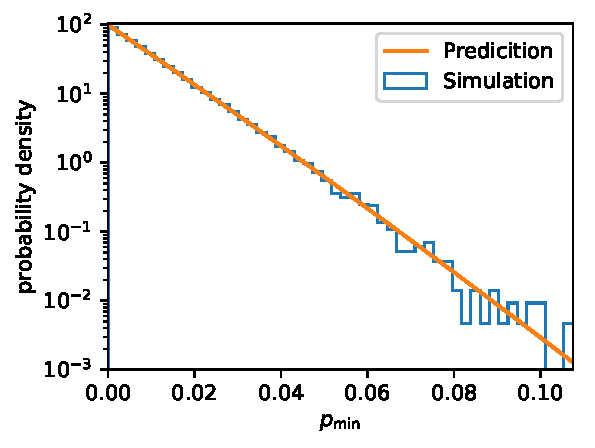
\includegraphics[width=0.5\textwidth]{minimal_pvalues}
    \caption{Minimal $p$-values from \num{100000} pseudo-experiments using $N = \num{100}$.}
    \label{fig:minimal_pvalues}
\end{figure}

One additional study on the probability density is to calculate the expected minimal value of $N$ uniform $p$-values:
\begin{equation}
    \langle p \rangle = \int_0^1 N \cdot \left(1-p\right)^{N-1} \cdot p \dd p = \frac{1}{N+1}
\end{equation}

\newpage
\section{Derivation of the Log-Normal $p$-value}
\label{app:lognormal_derivation}

Through the systematic uncertainties, the total number of events is scaled by an unknown factor $X$, which is a random variable that emerges as product of multiple other random variables $x_i$.
In the following section illustrates a derivation on how $X$ is distributed.

First, the product can be rewritten in terms of a sum within an exponential distribution:
\begin{equation}
    X = \prod_i x_i = \prod_i \exp(\ln(x_i)) = \exp(\sum_i \ln(x_i))
\end{equation}
$\ln(x_i)$ is a random variable, and the central limit theorem implies that the sum is distributed according to the normal distribution.
\begin{equation}
    Y \defeq \sum_i \ln(x_i) \Rightarrow X = \exp(Y) \text{ and } f_Y(y) = \frac{1}{\sqrt{2\pi}\sigma} \exp(-\frac{1}{2}\left(\frac{y-\mu}{\sigma}\right)^2)
\end{equation}
After defining $Y$ as the normally distributed variable with the probability density $f_Y(y)$, one introduces a new unknown probability density function $g_X(x)$:
\begin{equation}
    f_Y(y) \: \dd y \eqdef g_X(x) \: \dd x 
\end{equation}
Finally, one can insert all definitions, calculate the derivative and write the distribution function dependent of $x$:
\begin{align}
    g_X(x) &= f_Y(y) \: \dv{y}{x} \\
    &= f_Y(\ln{x}) \: \dv{\ln{x}}{x} \\
    &= f_Y(\ln{x}) \: \frac{1}{\abs{x}} \\
    &= \frac{1}{\sqrt{2\pi}\sigma\abs{x}} \exp(-\frac{1}{2}\left(\frac{\ln{x}-\mu}{\sigma}\right)^2)
\end{align}
The result is known as \emph{log-normal distribution} and is the probability density function of a product of random variables.

By performing two substitutions, a parametrization with a more meaningful interpretation is obtained:
\begin{equation}
    \sigma \rightarrow \ln{k} = \ln(1 + \sigma/x_0) \text{ and } \mu \rightarrow \ln{x_0}
    \label{eq:log_normal_substitution}
\end{equation}
\begin{equation}
    g_X(x) = \frac{1}{\sqrt{2\pi}\abs{x}\ln{k}} \exp(-\frac{1}{2}\left(\frac{\ln(x/x_0)}{\ln{k}}\right)^2)
\end{equation}

Here, $x_0$ is the expected value of $x$ and $k = 1 + \sigma/\mu$ is the relative uncertainty on $x_0$.

\newpage
\section{$Z$-score and $p$-value}
\label{app:z_score}

The probability $p$ associated with a $Z$-score is the cumulative tail probability of a normal distribution at $Z$ standard deviations from the mean:
\begin{equation}
    p = \frac{1}{\sqrt{2 \pi}}\int_Z^{\infty} \exp\left(-\frac{x^2}{2}\right) \text{d}x
\end{equation}

This yields the conversion formulas:
\begin{equation}
    p = \frac{1}{2} \left(1 - \text{erf}\left(\frac{Z}{\sqrt{2}}\right) \right) \Leftrightarrow Z = \sqrt{2} \cdot \text{erf}^{-1} \left( 1 - 2 p \right) 
\end{equation}

A table of values computed according to this formula can be found in \fref{tab:z_score_table}.

\begin{table}
    \small
    \def\arraystretch{1}
    \centering
    \begin{tabular}{S[table-figures-decimal = 1] S[table-figures-decimal = 6]}
\toprule
{$Z$} & {$p$} \\
\midrule
0.000000 & 0.500000 \\
0.100000 & 0.460172 \\
0.200000 & 0.420740 \\
0.300000 & 0.382089 \\
0.400000 & 0.344578 \\
0.500000 & 0.308538 \\
0.600000 & 0.274253 \\
0.700000 & 0.241964 \\
0.800000 & 0.211855 \\
0.900000 & 0.184060 \\
1.000000 & 0.158655 \\
1.100000 & 0.135666 \\
1.200000 & 0.115070 \\
1.300000 & 0.096800 \\
1.400000 & 0.080757 \\
1.500000 & 0.066807 \\
1.600000 & 0.054799 \\
1.700000 & 0.044565 \\
1.800000 & 0.035930 \\
1.900000 & 0.028717 \\
2.000000 & 0.022750 \\
2.100000 & 0.017864 \\
2.200000 & 0.013903 \\
2.300000 & 0.010724 \\
2.400000 & 0.008198 \\
\bottomrule
\end{tabular}
\hspace{1em}
\begin{tabular}{S[table-figures-decimal = 1] S[table-figures-decimal = 6]}
\toprule
{$Z$} & {$p$} \\
\midrule
2.500000 & 0.006210 \\
2.600000 & 0.004661 \\
2.700000 & 0.003467 \\
2.800000 & 0.002555 \\
2.900000 & 0.001866 \\
3.000000 & 0.001350 \\
3.100000 & 0.000968 \\
3.200000 & 0.000687 \\
3.300000 & 0.000483 \\
3.400000 & 0.000337 \\
3.500000 & 0.000233 \\
3.600000 & 0.000159 \\
3.700000 & 0.000108 \\
3.800000 & 0.000072 \\
3.900000 & 0.000048 \\
4.000000 & 0.000032 \\
4.100000 & 0.000021 \\
4.200000 & 0.000013 \\
4.300000 & 0.000009 \\
4.400000 & 0.000005 \\
4.500000 & 0.000003 \\
4.600000 & 0.000002 \\
4.700000 & 0.000001 \\
4.800000 & 0.000001 \\
4.900000 & 0.000000 \\
\bottomrule
\end{tabular}
    \caption{Conversion table for $Z$-score to a one tailed $p$-value.}
    \label{tab:z_score_table}
\end{table}

\newpage
\section{MUSiC Workflow}
\label{app:music_workflow}
\begin{figure}
    \centering
    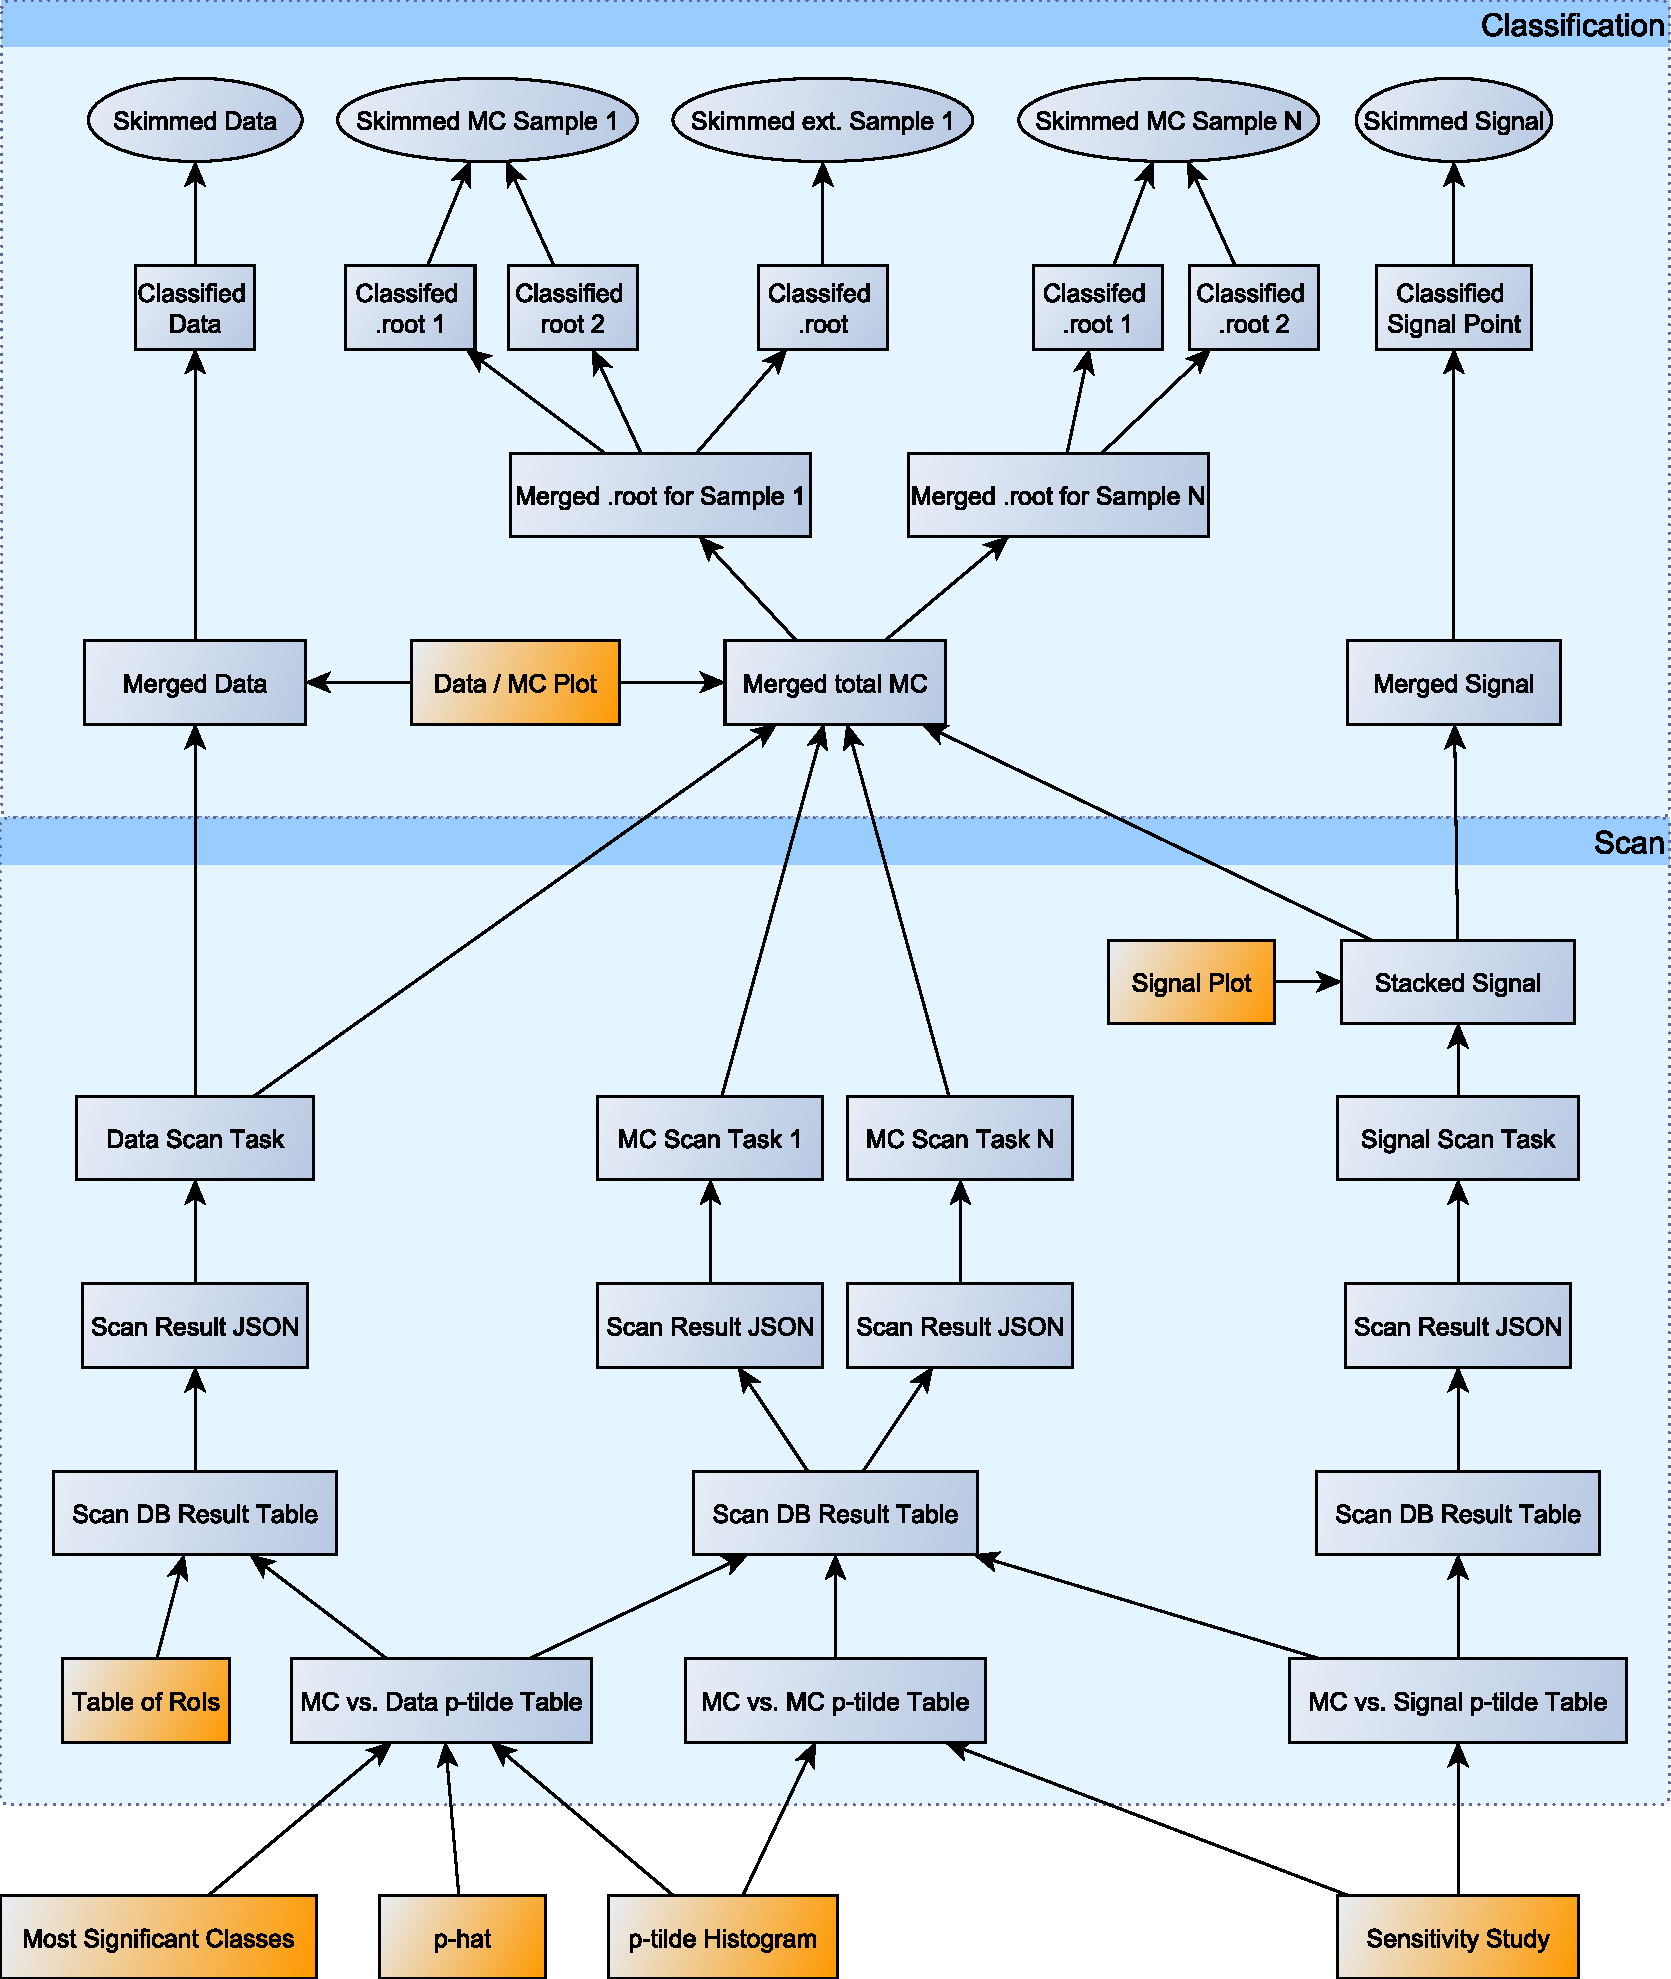
\includegraphics[width=\textwidth]{../music-workflow}
    \caption{Illustration of the dependencies of intermediate products during the analysis. Chronologically, the analysis starts at the top by classifying preprocessed ("skimmed") data and simulation samples. In the following steps, the classified samples are merged into a consistent set and the search for deviations is executed. Eventually, the results are stored in a database file and statistical inference is applied.}
    \label{fig:music_workflow}
\end{figure}

\newpage
\section{Performance of the Lookup-Table}
\label{app:lut_performance}

The performance of the \acf{LUT} is evaluated by applying the automated search on \ac{SM} pseudo-experiments with and without a \ac{LUT}. The classification output contains \num{4297} event classes, including event classes with \Pqb-tagged jets. The pseudo-experiments are generated on the \sumpT kinematic distribution.

The \ac{LUT} under evaluation is \SI{80}{\mega\byte} in size. The performance is measured by wall-time, therefore is subject to small deviations ($\pm \SI{3}{\percent}$), e.g. due to other processes using the same core.
The test is performed twice, on \num{10} (\fref{tab:lut_performance_10}) and \num{100} (\fref{tab:lut_performance_100}) pseudo-experiments, to indicate scaling behavior.

\begin{table}
    \centering
    \small
    \begin{tabular}{l l l}
        \toprule
        & without \ac{LUT} & with \ac{LUT} \\
        \midrule
        pseudo exp. generation & \SI{5}{\second} & \SI{5}{\second} \\
        region building / veto & \SI{1373}{\second} & \SI{1337}{\second} \\
        number of regions & \multicolumn{2}{c}{\num{223877750}} \\
        number of \TS values & \multicolumn{2}{c}{\num{92503930}} \\
        \ac{LUT} hits & - & \num{86681242} (\SI{93.7}{\percent}) \\
        time spent calculating \TS values & \SI{5220}{\second} (\SI{56}{\micro\second} per \TS) & \SI{561}{\second} (\SI{6}{\micro\second} per \TS) \\
        other & \SI{910}{\second} & \SI{1397}{\second} \\        
        \midrule
        total time & \SI{7517}{\second} & \SI{3300}{\second} \\
        \bottomrule
    \end{tabular}
    \caption{Performance results on the automated search on \num{4297} event classes, \num{10} pseudo-experiments on the \sumpT distribution. All listed durations express wall-time.}
    \label{tab:lut_performance_10}
\end{table}

%
%[8:01 PM] Jonas Lieb: LUT timing results!
%[8:01 PM] Jonas Lieb: 1. Ohne Lookuptable
%[8:01 PM] Jonas Lieb:
%    == RAW TIMING ==
%                            dicing:          4.7
%                            pValue:       5220.7
%                        roiFinding:       6593.6
%    ===============
%    == RAW STATS ==
%                          p-values:     92503930
%          skip: (classic) coverage:      4195355
%           skip: adaptive coverage:     13600580
%                       skip: empty:     30089330
%      skip: leading bg is negative:      1426160
%          skip: leading bg missing:     10553750
%              skip: low statistics:     13859140
%                 skip: negative MC:      1223625
%        skip: too much negative bg:      5547480
%                     total regions:    223877750
%    ===============
%    Total RoI-finding time: 6593.65s (1.83157h)
%    Time per p-value: 56.4377us
%[8:01 PM] Jonas Lieb: 2. Mit Lookuptable
%[8:01 PM] Jonas Lieb:
%    == RAW TIMING ==
%                            dicing:          4.7
%                            pValue:        561.3
%                        roiFinding:       1898.2
%    ===============
%    == RAW STATS ==
%                          lut: hit:     86681242
%                         lut: miss:      5822688
%                          p-values:     92503930
%          skip: (classic) coverage:      4182300
%           skip: adaptive coverage:     13600580
%                       skip: empty:     30089330
%      skip: leading bg is negative:      1426160
%          skip: leading bg missing:     10553750
%              skip: low statistics:     13859140
%                 skip: negative MC:      1236680
%        skip: too much negative bg:      5547480
%                     total regions:    223877750
%    ===============
%    Total RoI-finding time: 1898.24s (0.527288h)
%    Time per p-value: 6.06811us
%    LUT Hit percentage: 93.7 %
%[8:02 PM] Jonas Lieb: War jetzt ein voller SM-only scan, SumPt, bJets, lokal, 10 Pseudo-Experimente pro Klasse
%

\begin{table}
    \centering
    \small
    \begin{tabular}{l l l}
        \toprule
        & without \ac{LUT} & with \ac{LUT} \\
        \midrule
        pseudo exp. generation & \SI{33}{\second} & \SI{37}{\second} \\
        region building / veto & \SI{13520}{\second} & \SI{13365}{\second} \\
        number of regions & \multicolumn{2}{c}{\num{2238777500}} \\
        number of \TS values & \multicolumn{2}{c}{\num{925039300}} \\
        \ac{LUT} hits & - & \num{862902004} (\SI{93.3}{\percent}) \\
        time spent calculating \TS values & \SI{53746}{\second} (\SI{58}{\micro\second} per \TS) & \SI{6165}{\second} (\SI{7}{\micro\second} per \TS) \\
        other & \SI{1022}{\second} & \SI{1615}{\second} \\
        \midrule
        total time & \SI{68321}{\second} & \SI{21182}{\second} \\
        \bottomrule
    \end{tabular}
    \caption{Performance results on the automated search on \num{4297} event classes, \num{100} pseudo-experiments on the \sumpT distribution. All listed durations express wall-time.}
    \label{tab:lut_performance_100}
\end{table}
%
%without LUT
%== RAW TIMING ==
%                        dicing:         33.4
%                        pValue:      53746.6
%                    roiFinding:      67266.9
%===============
%== RAW STATS ==
%                      p-values:    925039300
%      skip: (classic) coverage:     41893018
%       skip: adaptive coverage:    136005800
%                   skip: empty:    300893300
%  skip: leading bg is negative:     14261600
%      skip: leading bg missing:    105537500
%          skip: low statistics:    138591400
%             skip: negative MC:     12296782
%    skip: too much negative bg:     55474800
%                 total regions:   2238777500
%===============
%Total RoI-finding time: 67266.9s (18.6853h)
%Time per p-value: 58.1019us
% wall time: 68321s
%
%with LUT
%
%== RAW TIMING ==
%                        dicing:         36.6
%                        pValue:       6165.1
%                    roiFinding:      19530.9
%===============
%== RAW STATS ==
%                      lut: hit:    862902004
%                     lut: miss:     62137296
%                      p-values:    925039300
%      skip: (classic) coverage:     41885803
%       skip: adaptive coverage:    136005800
%                   skip: empty:    300893300
%  skip: leading bg is negative:     14261600
%      skip: leading bg missing:    105537500
%          skip: low statistics:    138591400
%             skip: negative MC:     12303997
%    skip: too much negative bg:     55474800
%                 total regions:   2238777500
%===============
%Total RoI-finding time: 19530.9s (5.42526h)
%Time per p-value: 6.66467us
%LUT Hit percentage: 93.3 %
% Wall time: 21182s




\newpage
\section{Adapted Distributions for Coverage Tests}
\label{app:coverage_uncertainty}

A probability distribution parameterized by $\mu$ and $\sigma$ will in general not assign the same $p$-value to the value $x$ as the same distribution would do if it were parametrized by $x$ and $\sigma$ for the value $\mu$. This quite obvious fact becomes important during coverage testing: The pseudo-experiments generate a value \Nmc from a distribution usually parametrized by \Ntrue, but then in the following a distribution around \Nmc is used in the evaluation of the significance.

In this section, I want to regard the special cases of a normal probability distribution and a log-normal distribution and derive a formula for adapting the distribution width parameter $\sigma$ such that the $p$-value to include \Ntrue in a (log-)normal distribution parametrized around \Nmc will remain the same as for \Nmc parametrized by \Ntrue. However, some of the ideas mentioned here can be adapted to other distributions too. 

We start by rephrasing the problem as an equation:
\begin{equation}
    \Pr(x \leq \Nmc | \Ntrue, \sigma) = \Pr(x \geq \Ntrue | \Nmc, \sigma')
\end{equation}

This equation can also be graphically illustrated as in \fref{fig:coverage_distributions}. The blue dashed distribution indicates the initial probability distribution which is used to generate the pseudo-experiments. The orange distribution is the resulting distribution used to calculate the $p$-value, which has been modified according to the recipe from this chapter, in order to keep the integrals (circled and cross-hatched areas) equal.

\begin{figure}
    \centering
    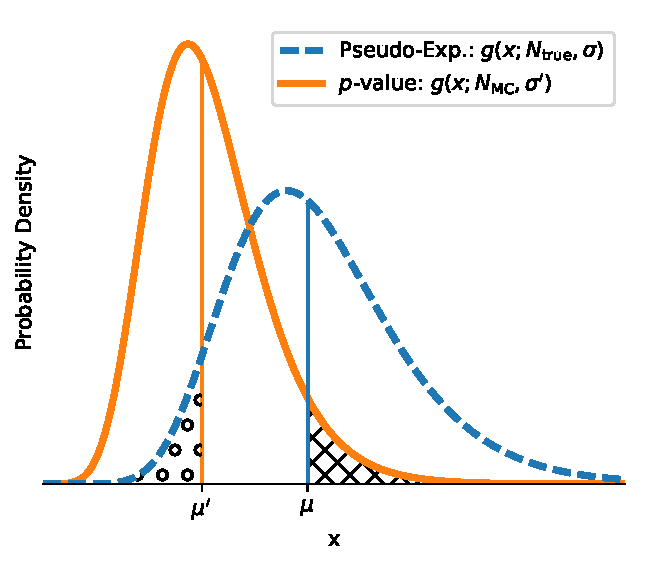
\includegraphics[width=0.5\textwidth]{coverage/coverage_distributions}
    \caption{Difference in widths of distributions while keeping the $p$-values constant.}
    \label{fig:coverage_distributions}
\end{figure}

Now, let $g(x | \Ntrue, \sigma)$ be the distribution from which the pseudo-experiments are drawn and $G(x | \Ntrue; \sigma)$ its cumulative distribution function. The left-hand-side now spells out:
\begin{equation}
    \Pr(x \leq \Nmc | \Ntrue, \sigma) = \int_0^{\Nmc} g(x | \Ntrue, \sigma) \dd{x} = G(\Nmc | \Ntrue, \sigma) - G(0 | \Ntrue, \sigma)
\end{equation}

The right hand side consists of the distribution used for calculating the $p$-value:
\begin{equation}
    \Pr(x \geq \Ntrue | \Nmc, \sigma) = \int_\Ntrue^\infty g(x | \Nmc, \sigma') \dd{x} = G(\infty | \Nmc, \sigma') - G(\Ntrue | \Nmc, \sigma')
\end{equation}
Since $G$ is a cumulative distribution function, one can substitute $G(0) = 0$ and $G(\infty) = 1$ and set both sides equal:
\begin{equation}
    G(\Nmc | \Ntrue, \sigma) = 1 - G(\Ntrue | \Nmc, \sigma')
\end{equation}
The width adaption can now be specified by solving this equation for $\sigma'(\Ntrue, \Nmc, \sigma)$.

For this purpose, first a general solution for $\Phi(x)$, which is the cumulative distribution function of a standard normal distribution $\mathcal N(\mu=0, \sigma=1)$, is derived:

\begin{align}
    \Phi(x) &= 1 - \Phi(x') \\
    \Rightarrow x' &= \Phi^{-1}(1 - \Phi(x)) \\
    &= \sqrt{2} \erf^{-1}\left(2 \cdot \left[1 - \frac{1}{2} \left(1+\erf\left(\frac{x}{\sqrt{2}}\right)\right)\right]-1\right) \\
    %&= \sqrt{2}\erf^{-1}\left(2-1-\erf\left(\frac{x}{\sqrt{2}}\right)-1\right) \\
    &= \sqrt{2}\erf^{-1}\left(-\erf\left(\frac{x}{\sqrt{2}}\right)\right) \\
    &= \sqrt{2}\erf^{-1}\left(\erf\left(\frac{-x}{\sqrt{2}}\right)\right) \\
    &= -x
\end{align}

Here, it has been used that $\Phi$ can be expressed in terms of the error function, which in turn can be further expressed by an integral.
\begin{align}
    \Phi(x) &= \frac{1}{2} \left(1+\erf\left(\frac{x}{\sqrt{2}}\right)\right) \\
    \Phi^{-1}(x) &= \sqrt{2}\,\erf^{-1}(2x - 1) \\
    \erf(x) &= \frac{2}{\sqrt{\pi}} \int_0^x e^{-t^2} \dd{t}
\end{align}

The error function is odd, i.e. $\erf(-x) = -\erf(x)$.

\subsubsection{Normal Distribution}
A general normal distribution $\mathcal N(\mu, \sigma)$ has the following cumulative distribution function:
\begin{equation}
    G(\mu' | \mu, \sigma) = \Phi\left(\frac{\mu' - \mu}{\sigma}\right); \quad
    G(\mu | \mu', \sigma') = \Phi\left(\frac{\mu - \Nmc}{\sigma'}\right)
\end{equation}

One can now use the expression for $\Phi$ derived earlier to solve the initial equation:
\begin{align}
    \Phi\left(\frac{\Nmc - \Ntrue}{\sigma}\right) &= 1 - \Phi\left(\frac{\Ntrue - \Nmc}{\sigma'}\right) \\
    \Rightarrow \frac{\Nmc - \Ntrue}{\sigma} &= - \frac{\Ntrue - \Nmc}{\sigma'} \\
    \Rightarrow \sigma' &= \sigma
\end{align} 

The final result is that the width parameter does not have to be adapted for a normal distribution, which was expected (as it is symmetrical). 

\subsubsection{Log-Normal Distribution}
The argumentation for the log-normal distribution is similar. The cumulative distribution of the log-normal distribution is 
\begin{equation}
    G(x | \Ntrue, \sigma) = \Phi\left(\frac{\ln x - \Ntrue}{\sigma}\right)
\end{equation}

Following the same argumentation, one obtains that again $\sigma$ must be conserved. However, in contrast to the case of the normal distribution, $\sigma$ now only depends on the \emph{relative} uncertainty (see \fref{eq:log_normal_substitution}).

\subsubsection{Conclusion}
Overall, one can conclude that the distributions used for pseudo-experiment generation and evaluation of the $p$-value are not necessarily the same. In order to keep the probabilities to obtain \Ntrue from \Nmc after drawing \Nmc from \Ntrue the same, in case of the log-normal distribution, the absolute error has to be recomputed with the newly drawn \Nmc, such that the relative error remains the same. The normal property does not need such adaptation as it has the decent property of being symmetrical.

\newpage
\section{Comparison of Coverage Results with Thesis by Stefan Schmitz}
\label{app:coverage_schmitz}

\begin{figure}
    \centering
    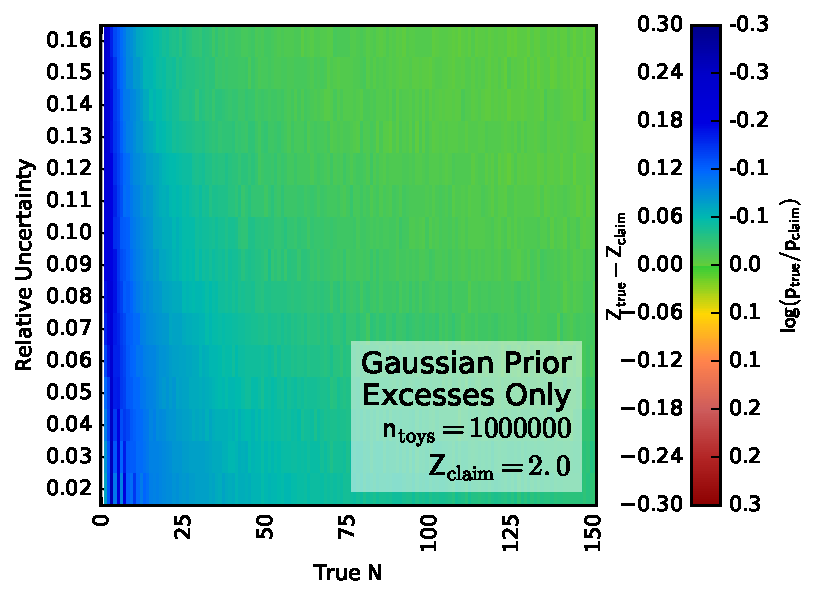
\includegraphics[width=0.8\textwidth]{coverage/coverage_excess_normal_schmitz}
    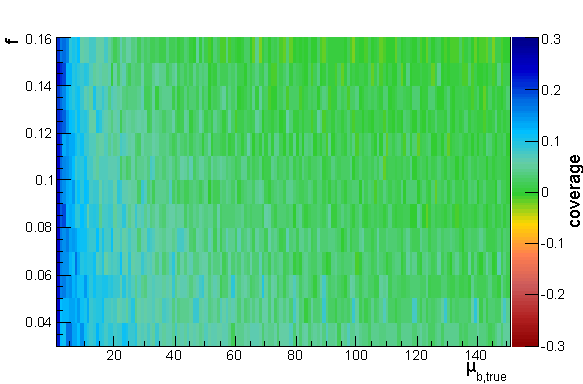
\includegraphics[width=0.8\textwidth]{schmitz_coverage}
    \caption{Comparison of my results (top) with \cite{Schmitz:ModelUnspecificSearch} (bottom). The test settings as well as plotting options have been chosen to match. From visual inspection I deduce that the results are very similar and therefore conclude that I can directly compare results from my implementation with the earlier thesis.}
    \label{fig:coverage_schmitz}
\end{figure}

\newpage
\section{Additional Coverage Results for \TS and \TSprime}
\label{app:coverage_additional_results}

\begin{figure}
    \centering
    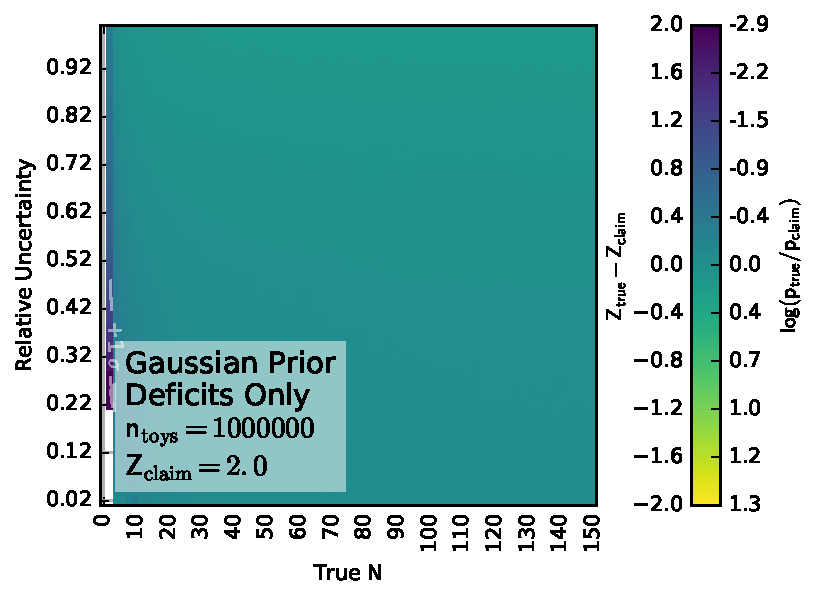
\includegraphics[width=0.9\textwidth]{coverage/coverage_deficit_normal_lin}
    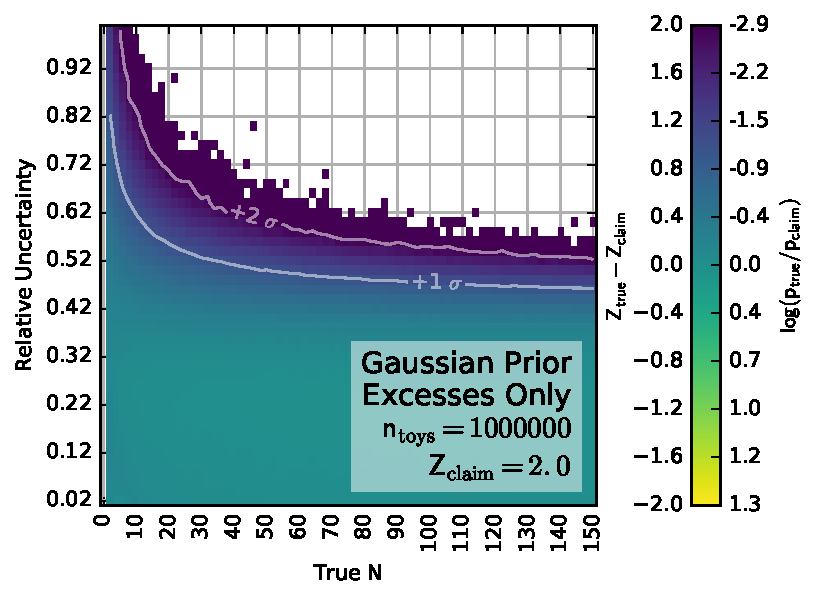
\includegraphics[width=0.9\textwidth]{coverage/coverage_excess_normal_lin}
    \caption{Results of the coverage study of \TS, similar to \fref{fig:coverage_normal}, but evaluated on a non-logarithmic grid.}
\end{figure}

\begin{figure}
    \centering
    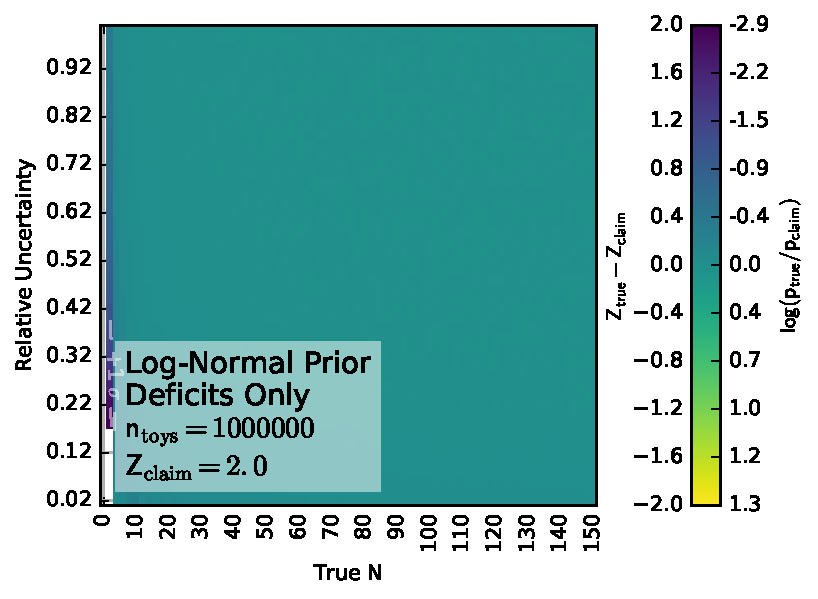
\includegraphics[width=0.9\textwidth]{coverage/coverage_deficit_lognormal_lin}
    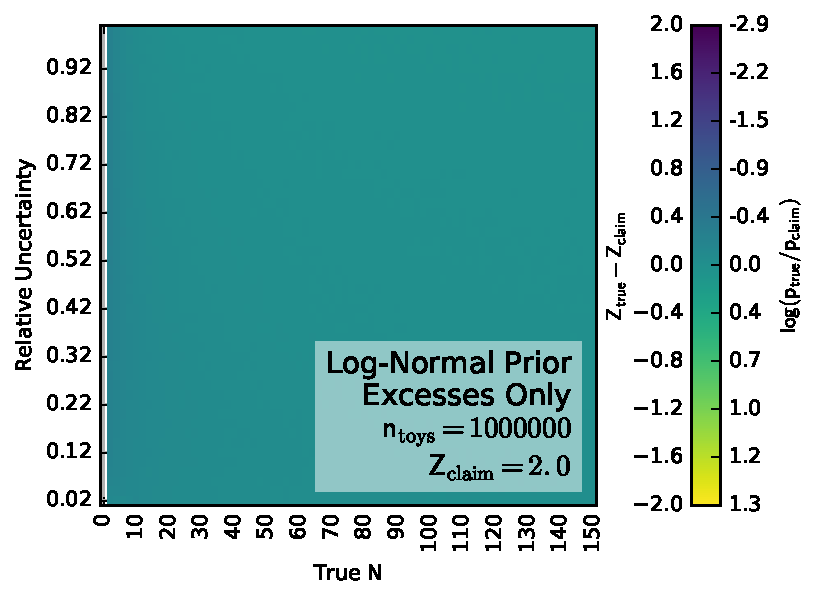
\includegraphics[width=0.9\textwidth]{coverage/coverage_excess_lognormal_lin}
    \caption{Results of the coverage study of \TSprime, similar to \fref{fig:coverage_lognormal}, but evaluated on a non-logarithmic grid.}
\end{figure}